\documentclass[border=3pt]{standalone}
% Shared TikZ styles for the Ch. 3–8 diagrams (standalone PDFs); extends the Ch. 1 palette (s1_vs_llm_common.tex).
\usepackage[T1]{fontenc}
\usepackage{lmodern}
\usepackage[english]{babel}
\usepackage{amsmath,amssymb}
\usepackage{tikz}
\usetikzlibrary{shapes.geometric,shapes.misc,positioning,fit,arrows.meta,calc,backgrounds,decorations.pathreplacing,patterns}
\definecolor{ioFill}{HTML}{F1F0EC}\definecolor{ioLine}{HTML}{52514E}
\definecolor{modFill}{HTML}{E8F1FB}\definecolor{modLine}{HTML}{2A78D6}
\definecolor{decFill}{HTML}{ECE9F7}\definecolor{decLine}{HTML}{4A3AA7}
\definecolor{postFill}{HTML}{FFF6E0}\definecolor{postLine}{HTML}{EDA100}
\definecolor{okFill}{HTML}{EAF7F1}\definecolor{okLine}{HTML}{1BAF7A}
\definecolor{badFill}{HTML}{FDECEC}\definecolor{badLine}{HTML}{E34948}
\definecolor{nmFill}{HTML}{EFEAF8}\definecolor{nmLine}{HTML}{4A3AA7}
\definecolor{loopRed}{HTML}{E34948}\definecolor{clusterLine}{HTML}{9A9890}\definecolor{ink2}{HTML}{52514E}
\definecolor{orangeA}{HTML}{EB6834}
\tikzset{
  every node/.style={font=\small, align=center},
  io/.style={trapezium, trapezium left angle=72, trapezium right angle=108, trapezium stretches body,
             draw=ioLine, fill=ioFill, thick, inner sep=3pt, minimum height=2.4em},
  model/.style={rectangle, draw=modLine, fill=modFill, very thick, inner sep=4pt, minimum height=2.4em, text width=#1},
  model/.default=3.6cm,
  post/.style={rectangle, draw=postLine, fill=postFill, very thick, inner sep=4pt, minimum height=2.2em, text width=#1},
  post/.default=3.6cm,
  data/.style={cylinder, shape border rotate=90, aspect=0.18, draw=okLine, fill=okFill, very thick, inner sep=3pt, minimum height=2.6em, text width=#1},
  data/.default=2.4cm,
  decision/.style={diamond, aspect=2.1, draw=decLine, fill=decFill, very thick, inner sep=1pt},
  outcome/.style={rounded rectangle, draw=#1, thick, inner sep=4pt, minimum height=2em},
  arrow/.style={-{Latex[length=2mm]}, thick, ioLine},
  dashedarrow/.style={-{Latex[length=2mm]}, thick, ioLine, dashed},
  loop/.style={-{Latex[length=2.4mm]}, line width=1.4pt, loopRed},
  cluster/.style={draw=clusterLine, dashed, rounded corners=3pt, inner sep=7pt},
  clusterlabel/.style={font=\small\bfseries, text=ioLine},
  note/.style={font=\footnotesize, text=ink2},
  tok/.style={rectangle, draw=ioLine, fill=ioFill, thin, inner sep=2pt, minimum height=1.6em, font=\footnotesize},
  vmark/.style={rectangle, draw=orangeA, fill=postFill, thick, inner sep=2pt, minimum height=1.6em, font=\footnotesize\ttfamily},
}

\begin{document}
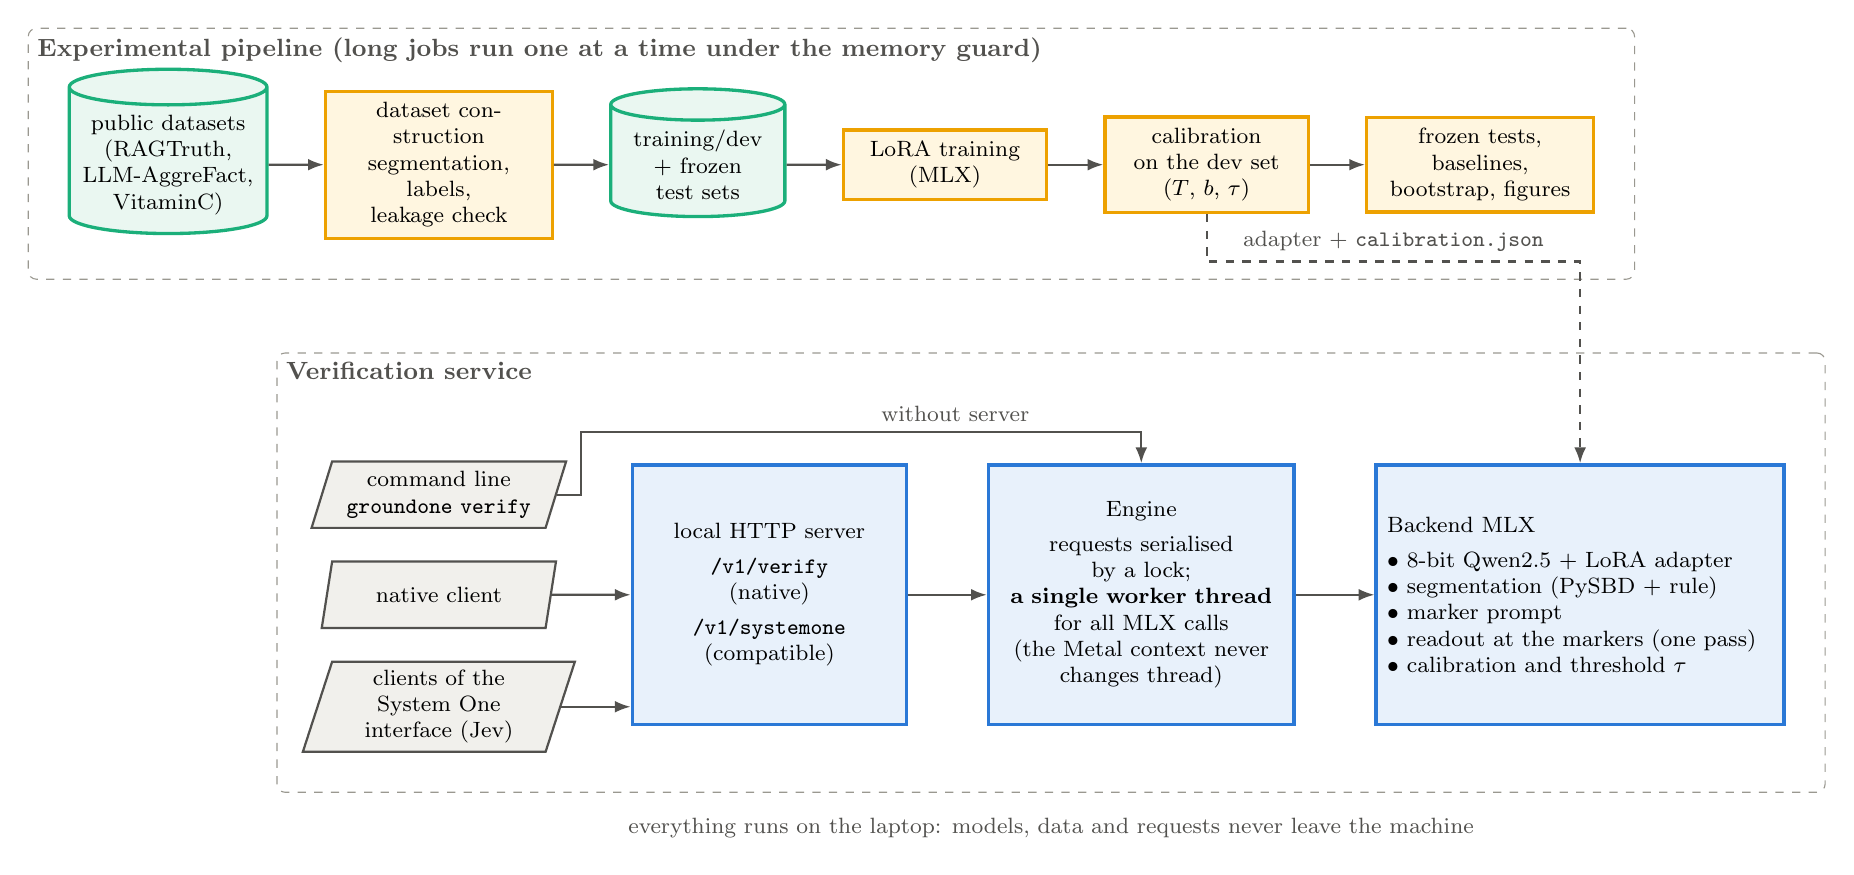
\begin{tikzpicture}[node distance=5mm]
  % ---------- offline pipeline ----------
  \node[data=2.3cm, font=\footnotesize] (raw) {public datasets\\(RAGTruth, LLM-AggreFact, VitaminC)};
  \node[post=2.6cm, right=7mm of raw, font=\footnotesize] (build) {dataset construction\\segmentation, labels,\\leakage check};
  \node[data=2.0cm, right=7mm of build, font=\footnotesize] (frozen) {training/dev\\+ frozen\\test sets};
  \node[post=2.3cm, right=7mm of frozen, font=\footnotesize] (train) {LoRA training\\(MLX)};
  \node[post=2.3cm, right=7mm of train, font=\footnotesize] (calib) {calibration\\on the dev set\\($T$, $b$, $\tau$)};
  \node[post=2.6cm, right=7mm of calib, font=\footnotesize] (eval) {frozen tests, baselines,\\bootstrap, figures};
  \foreach \a/\b in {raw/build,build/frozen,frozen/train,train/calib,calib/eval} \draw[arrow] (\a) -- (\b);
  \begin{scope}[on background layer]
    \node[cluster, fit=(raw)(build)(frozen)(train)(calib)(eval), inner sep=5mm, label={[clusterlabel, anchor=north west]north west:Experimental pipeline (long jobs run one at a time under the memory guard)}] (off) {};
  \end{scope}
  % ---------- serving ----------
  \node[io, text width=2.5cm, below=28mm of build, font=\footnotesize] (cli) {command line\\\texttt{groundone verify}};
  \node[io, text width=2.5cm, below=4mm of cli, font=\footnotesize] (cl1) {native client};
  \node[io, text width=2.5cm, below=4mm of cl1, font=\footnotesize] (cl2) {clients of the\\System One interface (Jev)};
  \node[model=3.2cm, right=10mm of cl1, minimum height=3.3cm, font=\footnotesize] (api) {local HTTP server\\[3pt]\texttt{/v1/verify}\\(native)\\[3pt]\texttt{/v1/systemone}\\(compatible)};
  \node[model=3.6cm, right=10mm of api, minimum height=3.3cm, font=\footnotesize] (eng) {Engine\\[3pt]requests serialised\\by a lock;\\\textbf{a single worker thread}\\for all MLX calls\\(the Metal context never\\changes thread)};
  \node[model=4.9cm, right=10mm of eng, minimum height=3.3cm, font=\footnotesize, align=left] (bk) {Backend MLX\\[3pt]$\bullet$ 8-bit Qwen2.5 + LoRA adapter\\$\bullet$ segmentation (PySBD + rule)\\$\bullet$ marker prompt\\$\bullet$ readout at the markers (one pass)\\$\bullet$ calibration and threshold $\tau$};
  \draw[arrow] (cli.east) -- ++(3mm,0) |- ([yshift=4mm]api.north) -| node[pos=0.25, above, note] {without server} (eng.north);
  \draw[arrow] (cl1) -- (api.west |- cl1);
  \draw[arrow] (cl2.east) -- (api.west |- cl2.east);
  \draw[arrow] (api) -- (eng);
  \draw[arrow] (eng) -- (bk);
  \begin{scope}[on background layer]
    \coordinate (topc) at ([yshift=9mm]api.north);
    \node[cluster, fit=(cli)(cl2)(api)(eng)(bk)(topc), inner sep=5mm, label={[clusterlabel, anchor=north west]north west:Verification service}] (srv) {};
  \end{scope}
  \draw[dashedarrow] (calib.south) -- ++(0,-6mm) -| node[pos=0.25, above, note] {adapter + \texttt{calibration.json}} (bk.north);
  \node[note, below=2mm of srv.south] {everything runs on the laptop: models, data and requests never leave the machine};
\end{tikzpicture}
\end{document}
